

% DK: I am not sure that this is a Pattern. It is a role for sure, but is it a solution to a problem? Maybe the name of the pattern is wrong. Something like Welcome Wagon? Something that evokes the response to the Newcomer.
\section{Newcomer}\label{sec:Newcomer}

\subsubsection*{Motivation} This pattern can help project participants be aware of the issues faced by newcomers, and cultivate a ``beginner's mind'' themselves.

\subsubsection*{Context}
% DK: This is an interesting point. I am not sure it is Context. Maybe Rationale?
When there's learning happening, it's because there is someone who is new to a topic, or to something about the topic.

\subsubsection*{Forces}~
\begin{tabular}[t]{p{.8\textwidth}@{\hspace{.03\textwidth}}c}
\textbf{Individuation}: each person learning optimally is what's best for the community. & {\icon \symbol{"0021E5}} \\
\textbf{Mutuality}: our individuality does not isolate us from one another, but draws us together. & 
{\icon \symbol{"002180}}%{\icon \symbol{"002117}}
\\
\end{tabular}

\subsubsection*{Problem} Newcomers can feel overwhelmed by the amount of things to learn.  They
often don't know where to start.  They may have a bunch of ideas that the
oldtimers have never considered -- or they may think they have new
ideas, which are actually a different take on an old idea; see
\patternname{Reduce, reuse, recycle}. People who are new to the project can tell you what makes their participation difficult.  Since you're learning as you go as well, you can ask yourself the same question: what aspects of this encounter are difficult for me?  

% DK: This seems a little spare
\subsubsection*{Solution}

Instead of thinking of newcomers as ``them'', and trying to provide
solutions, we focus on newcomers as ``us'' -- which makes the search
for solutions that much more urgent.  We permit ourselves to ask naive
questions.  We entertain vague ideas.  We add concreteness by trying
\patternname{A specific project}.  We may then genuinely turn to
others for help.
% OSS: What about action research?
% similar... not handholding but interactive
We aim to foster a culture in which the focus for everyone is on
addressing our own learning challenges rather than on ``providing''
solutions for others \cite{boud2005peer}.
%
As a general remark, the best practice for any newcomer is to be
prepared to engage immediately in action research
\cite{lewin1946action}.  Systematically take notes and gather data to
analyze and reflect upon later, leaving artifacts for future newcomers
to use and build upon in their own research cycle.  In practice this is a
lot to ask for someone just joining a group, but structuring
engagement so that it leads to collaborative research cycles
\emph{reflect}, \emph{plan}, \emph{act}, and \emph{observe} may be a
very effective way to improve the project and our collective
understanding.
% \footnote{\url{https://valenciacollege.edu/faculty/development/tla/actionResearch/ARP_softchalk/mobile_pages/index.html}}
Note that there is a partial parallel to the facets \emph{assess},
\emph{convene}, \emph{organize}, \emph{cooperate} from Figure
\ref{fig:connections}.  One method for doing the reflection\slash
assessment step is presented in the \patternname{Scrapbook} pattern.
Action research has previously been applied within institutions of
higher learning \cite{action-research-OU}, and elsewhere
\cite{trist1951some,bergold2012participatory}.
%
The peeragogical approach, based network-building,
leads to new ways of knowing and expanded access to
knowledge-production \cite{gilbert2012being,wagner2008new}.


% DK: I can empathize :+) I wonder if there is a pattern that is missing. Vision? A clear articulation about what the effort is for
%
\subsubsection*{Rationale} 
%
Sharing vulnerability and confusion gives us a chance to learn
together.  A newcomer's confusion about how best to get involved or
what the point of all this actually is may be due to a lack of
structure in the project \patternname{Roadmap}.  It points to places
where others in the project probably have something to learn.
%
%% In the words of Antoine de Saint-Exup\'ery:
%% ``If you want to build a boat, do not instruct the men to saw wood,
%% stitch the sails, prepare the tools and organize the work,
%% but make them long for setting sail and travel to distant lands.''

% DK: The resolution should describe the circumstance after applying the solution. This seems to be describe the circumstance without the solution.
\subsubsection*{Resolution}
An awareness of the difficulties that newcomers face can help us be
more compassionate to ourselves and others.  We strengthen the
community by supporting all participants' \textbf{individuation}.  We
have a better chance of making the project useful for others if we're
clear about how it is useful to \emph{us}.  By welcoming newcomers, we
enhance the sense of \textbf{mutuality} with people who have never
encountered the project before, and learn together with them.  The
facts start to become useful when we understand how people perceive
them \cite{freire1982creating}.

%% the concrete reality consists not only of concrete facts and
%% (physical) things, but also includes the ways in which the people
%% involved with these facts perceive them. Thus in the last analysis,
%% for me, the concrete reality is the connection between subjectivity
%% and objectivity, never objectivity isolated from subjectivity.

\subsubsection*{Example 1} Wikipedia \patternnameplural{Newcomer} can make use of resources that
include a ``Teahouse'' where questions are welcomed, a platform
extension that changes the user interface for new editors, and lots of
documentation.\footnote{\url{https://en.wikipedia.org/wiki/Wikipedia:Teahouse}}%
\textsuperscript{,}\footnote{\url{https://en.wikipedia.org/wiki/Wikipedia:GettingStarted}}%
\textsuperscript{,}\footnote{\url{https://en.wikipedia.org/wiki/Help:Editing}}
The efforts of exceptional newcomers may be given special
recognition.\footnote{\url{https://en.wikipedia.org/wiki/Template:The_New_Editor\%27s_Barnstar}}
Newcomer ``survival'' is of interest to the Wikimedia
Foundation.\footnote{\url{https://meta.wikimedia.org/wiki/Research:Newcomer_survival_models}}
However, ``Nearly all editors begin with a burst of activity, then
quickly tail off'' \cite{panciera2009wikipedians}.  The degree to
which those editors who are retained emphasize continuous upskilling
is somewhat less clear.  As regards learning their way around the
community, quantitative support exists \cite{panciera2009wikipedians}
for the claim that ``novice users learn the rules and conventions for
contributing both through observation and direct coaching from more
knowledgeable others'' \cite{bryant2005becoming}.

\begin{wrapfigure}{r}{.47\textwidth}
\vspace{-.9cm}
\begin{center}
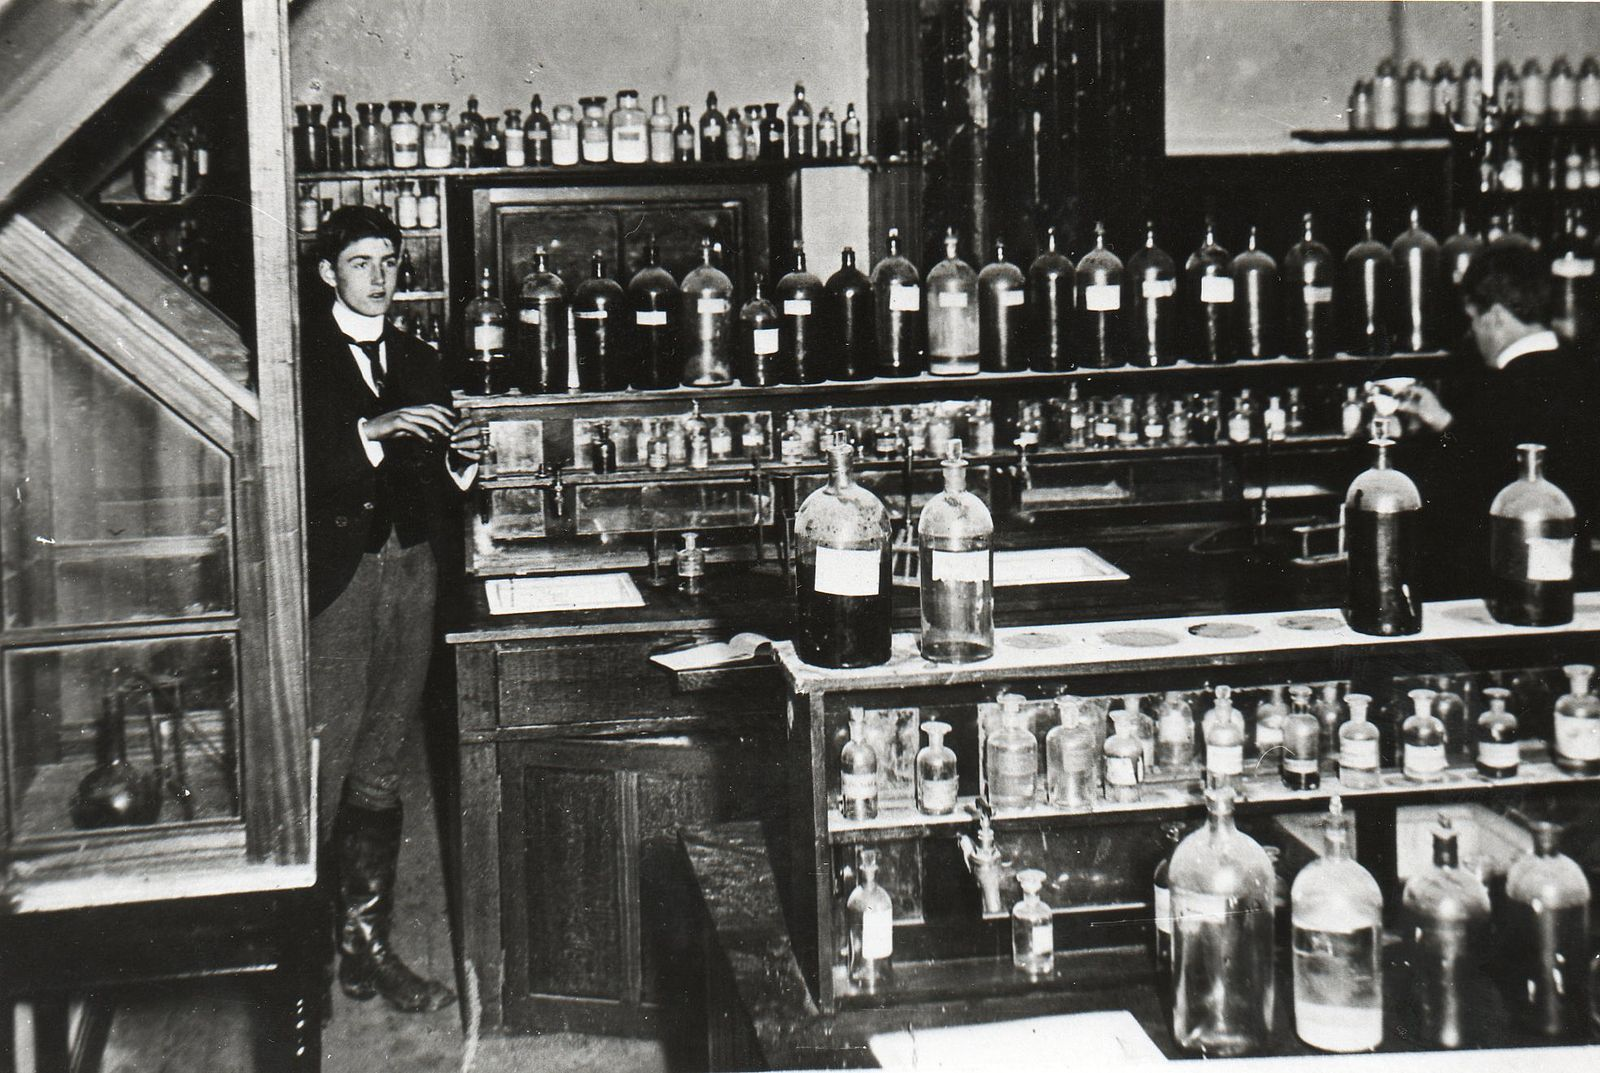
\includegraphics[width=.45\textwidth]{The_Science_Laboratory}
\end{center}
\vspace{-.5cm}
\caption{Science Laboratory, Aspatria Agricultural College, Cumberland, UK. 
% Public domain.
\label{science-laboratory}}
\vspace{-.9cm}
\end{wrapfigure}

\subsubsection*{Example 2} It will often be pragmatic to connect
\patternnameplural{Newcomer} with employment directly, so that
the future university may see a closer coupling of science and
industry than would be found in the old Science Hall.  Inspiration can
be drawn the London-based freelancing cooperative Founders\&Coders,
which is able to offer intensive training in web development at no
cost to successful applicants, on the basis that some trainees will
choose to join the cooperative as paying members later
on.\footnote{\url{http://www.foundersandcoders.com/academy/}}


\begin{framed}
\noindent 
\emph{What's Next in the Peeragogy Project}
\definecollection{NewcomerWN}
\begin{collectinmacro}{\NewcomerWN}{}{}
More detailed guides can show \patternnameplural{Newcomer}  how they can contribute and what to expect when they do. We should have different guides for different "user stories". We can start by listing some of the things we're currently learning about.
\end{collectinmacro}
\NewcomerWN
\end{framed}

\newpage
